\documentclass{beamer}
\usepackage{graphicx}
\usepackage{xcolor}
\usepackage{tikz}
\usepackage{amsmath}
\usepackage{pgfplots}
\pgfplotsset{compat=1.18}

\definecolor{purpleblue}{RGB}{80, 80, 180}
\definecolor{novelPurple}{RGB}{98, 54, 255}
\definecolor{softPurple}{RGB}{180, 170, 255}
\definecolor{softGray}{RGB}{235, 235, 245}
\definecolor{lightText}{RGB}{90, 90, 110}

\usetheme{Madrid}
\usecolortheme{dolphin}
\graphicspath{{static/course_materials/}{static/hard/}{./}}

\setbeamerfont{title}{size=\Large,series=\bfseries}
\setbeamerfont{frametitle}{size=\LARGE,series=\bfseries}
\setbeamercolor{frametitle}{fg=white, bg=novelPurple}
\setbeamercolor{title}{fg=white, bg=purpleblue}

\title[Test IV]{\textbf{Test IV}}
\author{\textbf{Jack Zeng}}
\institute{\textcolor{white}{\textbf{Novel Prep}}}
\date{\today}

\begin{document}

\begin{frame}
    \titlepage
    \vfill
    \begin{flushright}
        \textcolor{purpleblue}{\Huge \textbf{Novel Prep}}
    \end{flushright}
\end{frame}

\begin{frame}
    \begin{tikzpicture}[remember picture, overlay]
        \shade[top color=softPurple, bottom color=softGray]
            (current page.north west) rectangle (current page.south east);
        \node[align=center] at (current page.center) {
            {\Huge\bfseries\textcolor{purpleblue}{Novel Prep}} \\[0.5cm]
            {\Large\itshape\textcolor{lightText}{Phase 3 · Mock Exam Training}}
        };
    \end{tikzpicture}
\end{frame}

\begin{frame}{Overview}
    \tableofcontents
\end{frame}

\begin{frame}
\section{Test IV}
    \begin{tikzpicture}[remember picture, overlay]
        \shade[top color=softPurple, bottom color=softGray]
            (current page.north west) rectangle (current page.south east);
        \node[align=center] at (current page.center) {
            {\LARGE\bfseries\textcolor{purpleblue}{Test IV}} \\[0.5cm]
            {\Large\itshape\textcolor{lightText}{22 Module 2-style mock exam questions}}
        };
    \end{tikzpicture}
\end{frame}

% --- Question 1 ---
\begin{frame}{Question 1}
\small
In the system of equations below, \( c \) is a constant. If the system has no solution, what is the value of \( c \)?

\[
\begin{aligned}
y &= \frac{1}{2}x + 8 \\
y &= cx + 10
\end{aligned}
\]
\end{frame}
\begin{frame}{Answer 1}
\small
\textbf{Final Answer:} $\boxed{\dfrac{1}{2}}$
\end{frame}

% --- Question 2 ---
\begin{frame}{Question 2}
\small
To earn money for college, Avery works two part-time jobs: A and B. She earns \$10 per hour working at job A and \$20 per hour working at job B. In one week, Avery earned a total of \( s \) dollars for working at the two part-time jobs. The graph below represents all possible combinations of numbers of hours Avery could have worked at the two jobs to earn \( s \) dollars. What is the value of \( s \)?

\begin{center}
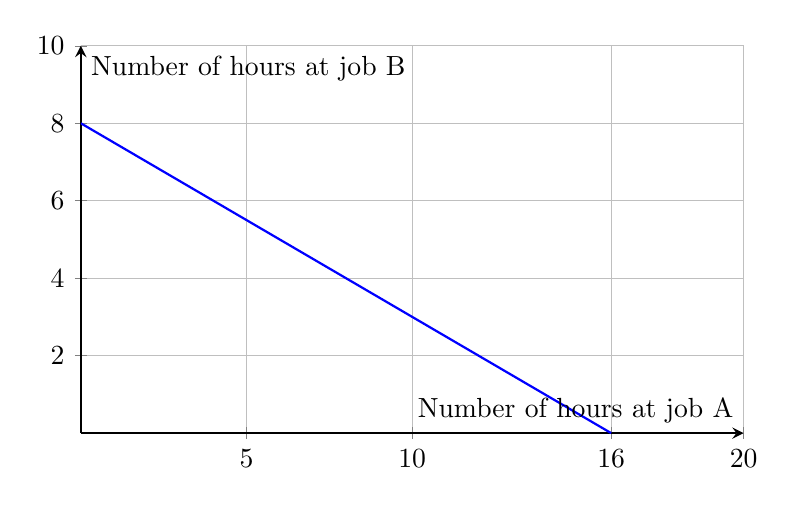
\begin{tikzpicture}
  \begin{axis}[
    width=10cm,
    height=6.5cm,
    xmin=0, xmax=20,
    ymin=0, ymax=10,
    axis lines=middle,
    xlabel={Number of hours at job A},
    ylabel={Number of hours at job B},
    xtick={0,5,10,16, 20},
    ytick={0,2,4,6,8,10},
    grid=major,
    thick
  ]
    % Plot the line y = 10 - 0.5x
    \addplot[
      domain=0:20,
      samples=100,
      thick,
      color=blue
    ] coordinates{(0,8)
    (16,0)};
  \end{axis}
\end{tikzpicture}
\end{center}
\vspace{0.35cm}
\begin{enumerate}
    \item[A.] 128
    \item[B.] 160
    \item[C.] 200
    \item[D.] 320
\end{enumerate}
\end{frame}
\begin{frame}{Answer 2}
\small
\textbf{Correct Answer:} B
\end{frame}

% --- Question 3 ---
\begin{frame}{Question 3}
\small
For each real number \( r \), which of the following points lies on the graph of each equation in the \( xy \)-plane for the given system?
\[
\begin{aligned}
2x + 3y &= 7 \\
10x + 15y &= 35
\end{aligned}
\]
\vspace{0.35cm}
\begin{enumerate}
    \item[A.] $\left(\frac{7}{5} + r, -\frac{7}{5} + 35 \right)$
    \item[B.] $\left(-\frac{3r}{2} + \frac{7}{2}, r \right)$
    \item[C.] $\left(r, \frac{2r}{3} + \frac{7}{3} \right)$
    \item[D.] $\left(r, -\frac{3r}{2} + \frac{7}{2} \right)$
\end{enumerate}
\end{frame}
\begin{frame}{Answer 3}
\small
\textbf{Correct Answer:} B
\end{frame}

% --- Question 4 ---
\begin{frame}{Question 4}
\small
The triangle inequality theorem states that the sum of any two sides of a triangle must be greater than the length of the third side. If a triangle has side lengths of $6$ and $12$, which inequality represents the possible lengths, $x$, of the third side of the triangle?
\vspace{0.35cm}
\begin{enumerate}
    \item[A.] $x < 18$
    \item[B.] $x > 18$
    \item[C.] $6 < x < 18$
    \item[D.] $x < 6 \text{ or } x > 18$
\end{enumerate}
\end{frame}
\begin{frame}{Answer 4}
\small
\textbf{Correct Answer:} C
\end{frame}

% --- Question 5 ---
\begin{frame}{Question 5}
\small
The expression \(\frac{x^{-2}y^{\frac{1}{2}}}{x^{\frac{1}{3}}y^{-1}}\), where \(x > 1\) and \(y > 1\), is equivalent to which of the following?
\vspace{0.35cm}
\begin{enumerate}
    \item[A.] \(\frac{\sqrt{y}}{\sqrt[3]{x^2}}\)
    \item[B.] \(\frac{y\sqrt{y}}{\sqrt[3]{x^{2}}}\)
    \item[C.] \(\frac{y\sqrt{y}}{x\sqrt{x}}\)
    \item[D.] \(\frac{y\sqrt{y}}{x^{2}\sqrt[3]{x}}\)
\end{enumerate}
\end{frame}
\begin{frame}{Answer 5}
\small
\textbf{Correct Answer:} D
\end{frame}

% --- Question 6 ---
\begin{frame}{Question 6}
\small
Which expression is equivalent to \(\frac{y + 12}{x - 8} + \frac{y(x - 8)}{x^2 y - 8xy}\) ?
\vspace{0.35cm}
\begin{enumerate}
    \item[A.] \(\frac{xy + y + 4}{x^2 y - 16x + 64xy}\)
    \item[B.] \(\frac{xy + 9 + 12}{x^2 y - 8xy + x - 8}\)
    \item[C.] \(\frac{xy^2 + 13xy - 8y}{x^2 y - 8xy}\)
    \item[D.] \(\frac{xy^2 + 13xy - 8y}{x^2 y - 16x^2 y + 64xy}\)
\end{enumerate}
\end{frame}
\begin{frame}{Answer 6}
\small
\textbf{Correct Answer:} C
\end{frame}

% --- Question 7 ---
\begin{frame}{Question 7}
\small
Solve for \(x\): \(\sqrt{2x + 6} + 4 = x + 3\)  
What is the solution set of the equation above?
\vspace{0.35cm}
\begin{enumerate}
    \item[A.] \(\{-1\}\)
    \item[B.] \(\{5\}\)
    \item[C.] \(\{-1, 5\}\)
    \item[D.] \(\{0, -1, 5\}\)
\end{enumerate}
\end{frame}
\begin{frame}{Answer 7}
\small
\textbf{Correct Answer:} B
\end{frame}

% --- Question 8 ---
\begin{frame}{Question 8}
\small
The formula  
\[
D = T - \frac{9}{25}(100 - H)
\]  
approximates the dew point \(D\) in Fahrenheit, given temperature \(T\) in Fahrenheit,  
and relative humidity \(H\%\), where \(H > 50\).  
Which of the following expresses \(H\) in terms of \(D\) and \(T\)?
\vspace{0.35cm}
\begin{enumerate}
    \item[A.] \(H = \frac{25}{9}(D - T) + 100\)
    \item[B.] \(H = \frac{25}{9}(D - T) - 100\)
    \item[C.] \(H = \frac{25}{9}(D + T) + 100\)
    \item[D.] \(H = \frac{25}{9}(D + T) - 100\)
\end{enumerate}
\end{frame}
\begin{frame}{Answer 8}
\small
\textbf{Correct Answer:} A
\end{frame}

% --- Question 9 ---
\begin{frame}{Question 9}
\small
\begin{center}
    

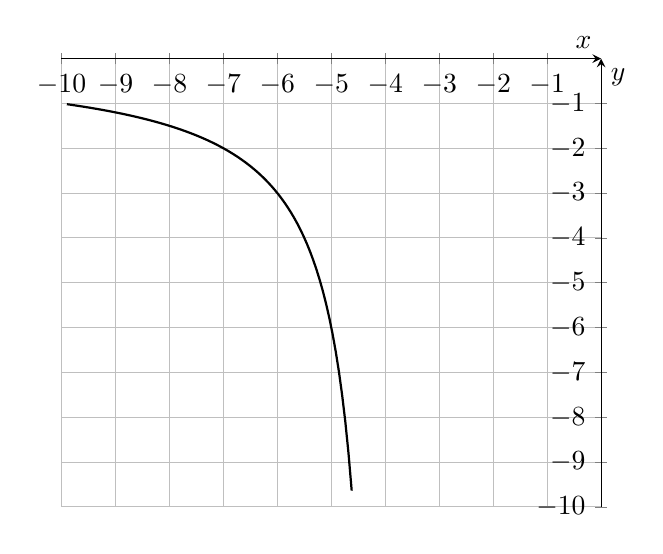
\begin{tikzpicture}
\begin{axis}[
    axis lines=center,
    xlabel=$x$, ylabel=$y$,
    xmin=-10, xmax=0,
    ymin=-10, ymax=0,
    xtick={-10,-9,...,0},
    ytick={-10,-9,...,0},
    samples=200,
    grid=major,
    domain=-9.9:1.9,
    restrict y to domain=-10:10
]
\addplot[thick, black] {6 / (x + 4)};
\end{axis}
\end{tikzpicture}

\end{center}

The rational function $f$ is defined by an equation in the form $f(x) = \dfrac{a}{x + b}$, where $a$ and $b$ are constants.  
The partial graph of $y = f(x)$ is shown.  
If $g(x) = f(x + 4)$, which equation could define function $g$?
\vspace{0.35cm}
\begin{enumerate}
    \item[A.] $g(x) = \dfrac{6}{x}$
    \item[B.] $g(x) = \dfrac{6}{x + 4}$
    \item[C.] $g(x) = \dfrac{6}{x + 8}$
    \item[D.] $g(x) = \dfrac{6(x - 4)}{x + 4}$
\end{enumerate}
\end{frame}
\begin{frame}{Answer 9}
\small
\textbf{Correct Answer:} C
\end{frame}

% --- Question 10 ---
\begin{frame}{Question 10}
\small
In the equation \(x^2 - 34x + c = 0\), \(c\) is a constant.  
The equation has no real solutions if \(c > n\).  
What is the least possible value of \(n\)?
\end{frame}
\begin{frame}{Answer 10}
\small
\textbf{Final Answer:} $\boxed{289}$
\end{frame}

% --- Question 11 ---
\begin{frame}{Question 11}
\small
The number $w$ is 110\% greater than the number $z$.  
The number $z$ is 55\% less than 50.  
What is the value of $w$?
\end{frame}
\begin{frame}{Answer 11}
\small
\textbf{Final Answer:} $\boxed{47.25}$
\end{frame}

% --- Question 12 ---
\begin{frame}{Question 12}
\small
The dot plot below shows the gas mileages, in miles per gallon, of 12 different cars.

\[
\begin{array}{cccccccccccc}
21 & 22 & 23 & 24 & 25 & 26 & 27 & 28 & 29 & 30 \\

\bullet & \bullet & \bullet & \bullet & \bullet & \bullet & \bullet & & & \bullet \\
& & \bullet & \bullet & \bullet & & & & & \\
& & & \bullet & & & & & &
\end{array}
\]

If the dot representing the car with the greatest gas mileage is removed from the dot plot,  
which of the following measures of the data set will decrease?

\begin{itemize}
\item[I.] The mean  
\item[II.] The median  
\item[III.] The standard deviation
\end{itemize}
\vspace{0.35cm}
\begin{enumerate}
    \item[A.] I only
    \item[B.] I and III only
    \item[C.] II and III only
    \item[D.] I, II, and III
\end{enumerate}
\end{frame}
\begin{frame}{Answer 12}
\small
\textbf{Correct Answer:} B
\end{frame}

% --- Question 13 ---
\begin{frame}{Question 13}
\small
In a psychological study, 600 college gymnasts were randomly selected and put in high-stakes competitions to determine whether they performed better under pressure.  
Based on the results of this study, it is estimated that 65\% of all college gymnasts perform better under pressure, with an associated margin of error of 4\%.  

Which of the following inferences can appropriately be drawn based on the given margin of error?
\vspace{0.35cm}
\begin{enumerate}
    \item[A.] The percentage of all college gymnasts who perform better under pressure is between 65\% and 69\%.
    \item[B.] Approximately 4\% of the college gymnasts in the study who performed better under pressure do not actually perform better under pressure.
    \item[C.] It is unlikely that the percentage of all college gymnasts who perform better under pressure is 60\%.
    \item[D.] It is not possible that the percentage of all college gymnasts who perform better under pressure is 70\%.
\end{enumerate}
\end{frame}
\begin{frame}{Answer 13}
\small
\textbf{Correct Answer:} C
\end{frame}

% --- Question 14 ---
\begin{frame}{Question 14}
\small
\begin{center}
    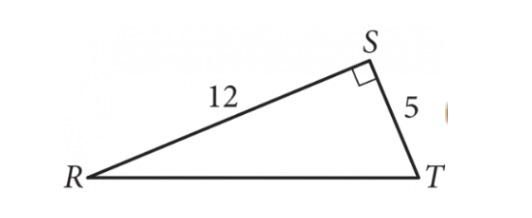
\includegraphics[width=0.55\linewidth]{hard_23_f13.png}
\end{center}

In triangle $RST$ above, point $W$ (not shown) lies on $\overline{RT}$. What is the value of $\cos(\angle RSW) - \sin(\angle WST)$?
\end{frame}
\begin{frame}{Answer 14}
\small
\textbf{Final Answer:} $\boxed{0}$
\end{frame}

% --- Question 15 ---
\begin{frame}{Question 15}
\small
A regular polygon has an interior angle that is 4 times the exterior angle plus 60 degrees.  
What is the number of sides of the polygon?
\vspace{0.35cm}
\begin{enumerate}
    \item[A.] 9
    \item[B.] 10
    \item[C.] 12
    \item[D.] 15
\end{enumerate}
\end{frame}
\begin{frame}{Answer 15}
\small
\textbf{Correct Answer:} D
\end{frame}

% --- Question 16 ---
\begin{frame}{Question 16}
\small
A circle in the \(xy\)-plane has equation  
\[
(x - 2.5)^2 + (y - 3.5)^2 = 225.
\]

Line \(p\) is tangent to the circle at point \((-6.5, C)\), where \(C\) is a constant.  
Which of the following could be the slope of line \(p\)?

\begin{itemize}
    \item[I.] \(-\frac{3}{4}\)
    \item[II.] \(\frac{3}{4}\)
    \item[III.] \(4/3\)
\end{itemize}
\vspace{0.35cm}
\begin{enumerate}
    \item[A.] I only
    \item[B.] I and II only
    \item[C.] I and III only
    \item[D.] I, II, and III
\end{enumerate}
\end{frame}
\begin{frame}{Answer 16}
\small
\textbf{Correct Answer:} B
\end{frame}

% --- Question 17 ---
\begin{frame}{Question 17}
\small
The function \(f\) is defined by \(f(x) = a^x - b\), where \(a\) and \(b\) are constants.  
In the \(xy\)-plane, the graph of \(y = f(x)\) passes through the points \((c, 7)\) and \((2c, 117)\), where \(c\) is a constant.  
Which of the following could be the value of \(b\)?
\end{frame}
\begin{frame}{Answer 17}
\small
\textbf{Final Answer:} $\boxed{4}$
\end{frame}

% --- Question 18 ---
\begin{frame}{Question 18}
\small
The given equation, where \(t\) is a positive constant, defines a circle in the \(xy\)-plane.  
The radius of this circle is \(\sqrt{41}\).  
What is the value of \(t\)?  
\[
2x^2 + 2y^2 + tx + ty - 78 = 0
\]
\end{frame}
\begin{frame}{Answer 18}
\small
\textbf{Final Answer:} $\boxed{4}$
\end{frame}

% --- Question 19 ---
\begin{frame}{Question 19}
\small
The table summarizes the distribution of heights, in inches (``in''), for 300 participants in a study. If a participant that is at most 71 inches tall is chosen at random, what is the probability that the participant was selected from Group 2?

\[
\begin{array}{|c|c|c|c|c|}
\hline
 & \text{48--59 in.} & \text{60--71 in.} & \text{72--83 in.} & \text{Total} \\
\hline
\text{Group 1} & 20 & 60 & 20 & 100 \\
\text{Group 2} & 10 & 75 & 15 & 100 \\
\text{Group 3} & 30 & 45 & 25 & 100 \\
\hline
\text{Total} & 60 & 180 & 60 & 300 \\
\hline
\end{array}
\]
\vspace{0.35cm}
\begin{enumerate}
    \item[A.] \(\dfrac{1}{4}\)
    \item[B.] \(\dfrac{17}{48}\)
    \item[C.] \(\dfrac{17}{60}\)
    \item[D.] \(\dfrac{17}{20}\)
\end{enumerate}
\end{frame}
\begin{frame}{Answer 19}
\small
\textbf{Correct Answer:} B
\end{frame}

% --- Question 20 ---
\begin{frame}{Question 20}
\small
The function \(f\) is defined as \(f(x) = x^2 + ax + b\), where \(a\) and \(b\) are positive integers. If the minimum value of \(f(x)\) is 7, which is a possible value of \(b\)?
\vspace{0.35cm}
\begin{enumerate}
    \item[A.] 6
    \item[B.] 7
    \item[C.] 8
    \item[D.] 9
\end{enumerate}
\end{frame}
\begin{frame}{Answer 20}
\small
\textbf{Correct Answer:} C
\end{frame}

% --- Question 21 ---
\begin{frame}{Question 21}
\small
The average annual energy cost for a certain home is \$4{,}334. The homeowner plans to spend \$25{,}000 to install a geothermal heating system. The homeowner estimates that the average annual energy cost will then be \$2{,}712. Which of the following inequalities can be solved to find \(t\), the number of years after installation at which the total amount of energy cost savings will exceed the installation cost?
\vspace{0.35cm}
\begin{enumerate}
    \item[A.] \(25{,}000 > (4{,}334 - 2{,}712)t\)
    \item[B.] \(25{,}000 < (4{,}334 - 2{,}712)t\)
    \item[C.] \(25{,}000 - 4{,}334 - 2{,}712t\)
    \item[D.] \(25000 > \dfrac{4332}{2712}t\)
\end{enumerate}
\end{frame}
\begin{frame}{Answer 21}
\small
\textbf{Correct Answer:} B
\end{frame}

% --- Question 22 ---
\begin{frame}{Question 22}
\small
Given the quadratic function  
\[
y = x^2 - 2ax + a \quad (a \ne 0)
\]  
passes through two points  
\[
A\left( \frac{a}{2}, y_1 \right), \quad B(3a, y_2),
\]  
which of the following statements is correct?
\vspace{0.35cm}
\begin{enumerate}
    \item[A.] There exists a real number \(a\) such that \(y_1 > a\).
    \item[B.] For all real numbers \(a\), \(y_1 > a\) is always true.
    \item[C.] There exists a real number \(a\) such that \(y_2 < 0\).
    \item[D.] For all real numbers \(a\), \(y_2 < 0\) is always true.
\end{enumerate}
\end{frame}
\begin{frame}{Answer 22}
\small
\textbf{Correct Answer:} C
\end{frame}

\begin{frame}{}
    \begin{tikzpicture}[remember picture, overlay]
        \shade[top color=novelPurple!40, bottom color=white]
            (current page.north west) rectangle (current page.south east);
        \fill[white, opacity=0.15] (current page.center) circle (5cm);
        \foreach \x in {1,2,3,4,5} {
            \fill[novelPurple, opacity=0.12] (rand*10-5, rand*7-3.5) circle (0.1+\x*0.05);
        }
    \end{tikzpicture}
    \centering
    \vspace{5em}
    {\Huge \textbf{\textcolor{novelPurple}{Thank You!}}} \\[1em]
    {\large \textcolor{gray}{We appreciate your time and focus.}} \\[3em]
    {\LARGE \textbf{\textcolor{novelPurple}{\textsf{Novel Prep}}}}
    \vfill
\end{frame}

\end{document}
